\chapter{Wireless Fundamentals}\label{wireless-fundamentals}

\begin{itemize}
\tightlist
\item
  Although we will briefly look at other types of WIRELESS NETWORKS, in
  this section of the course we will be focusing on WIRELESS LANs using
  WI-FI
\item
  The STANDARDS we use for WIRELESS LANs are defined in IEEE 802.11
\item
  The term WI-FI is a trademark of the WI-FI ALLIANCE, not directly
  connected to the IEEE
\item
  The WI-FI ALLIANCE tests and certifies equipment for 802.11 standards
  compliance
\item
  However, WI-FI has become the common term that people use to refer to
  802.11 WIRELESS LANs and that term will be used through the course
  videos
\end{itemize}

\section{Wireless Networks}\label{wireless-networks}

\begin{itemize}
\tightlist
\item
  WIRELESS NETWORKS have some issues that we need to deal with
\end{itemize}

\begin{figure}
\centering
\pandocbounded{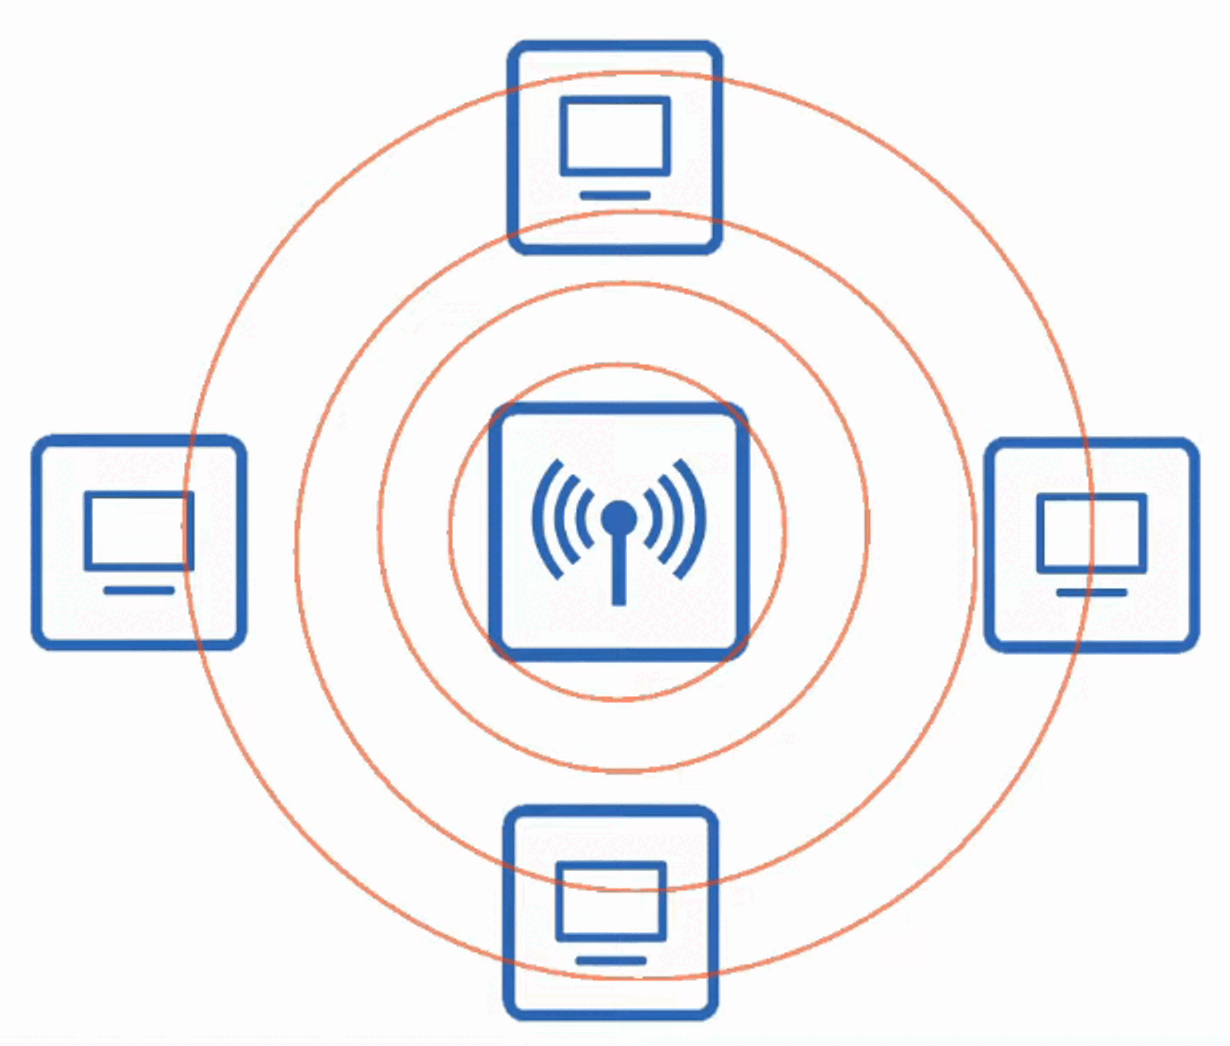
\includegraphics[keepaspectratio,alt={image}]{images/58-wireless-fundamentals/img-001.png}}
\end{figure}

\begin{enumerate}
\def\labelenumi{\arabic{enumi})}
\tightlist
\item
  ALL DEVICES within range receive ALL FRAMES, like DEVICES connected to
  an ETHERNET HUB
\end{enumerate}

\begin{itemize}
\item
  Privacy of DATA within the LAN is a greater concern
\item
  CSMA/CA (Carrier Sense Multiple Access with Collision Avoidance) is
  used to facilitate HALF-DUPLEX communications
\item
  CSMA / CD is used in WIRED NETWORKS to detect and recover from
  COLLISIONS
\item
  CSMA / CA is used in WIRELESS NETWORKS to avoid COLLISIONS
\item
  When using CSMA / CA, a DEVICE will wait for other DEVICES to STOP
  TRANSMITTING before it TRANSMITS DATA itself.
\end{itemize}

\begin{figure}
\centering
\pandocbounded{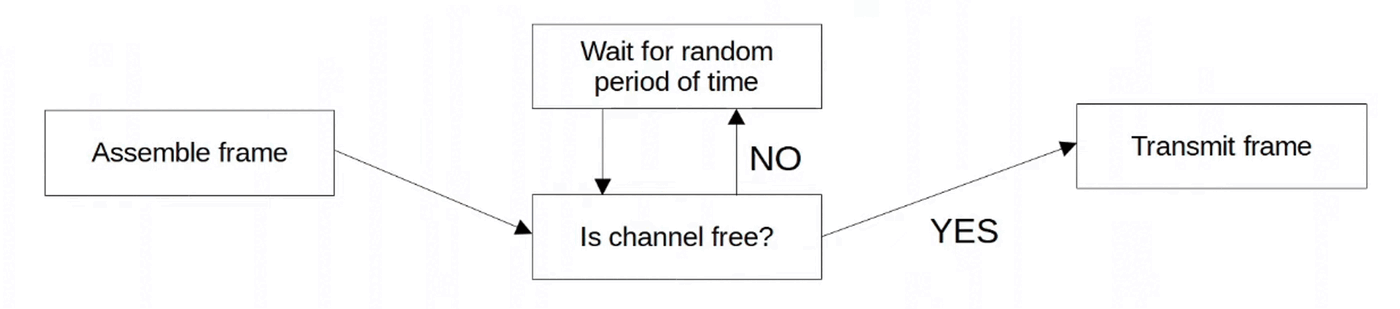
\includegraphics[keepaspectratio,alt={image}]{images/58-wireless-fundamentals/img-002.png}}
\end{figure}

\begin{enumerate}
\def\labelenumi{\arabic{enumi})}
\setcounter{enumi}{1}
\item
  WIRELESS COMMUNICATIONS are regulated by various INTERNATIONAL and
  NATIONAL bodies
\item
  WIRELESS SIGNAL COVERAGE AREA must be considered
\end{enumerate}

\begin{itemize}
\tightlist
\item
  Signal Range
\item
  Signal ABSORPTION, REFLECTION, REFRACTION, DIFFRACTION, and SCATTERING
\end{itemize}

\section{Signal Absorption}\label{signal-absorption}

\begin{itemize}
\tightlist
\item
  ABSOPTION happens when a WIRELESS SIGNAL PASSES THROUGH a material and
  is converted into HEAT, weakening the SIGNAL
\end{itemize}

\begin{figure}
\centering
\pandocbounded{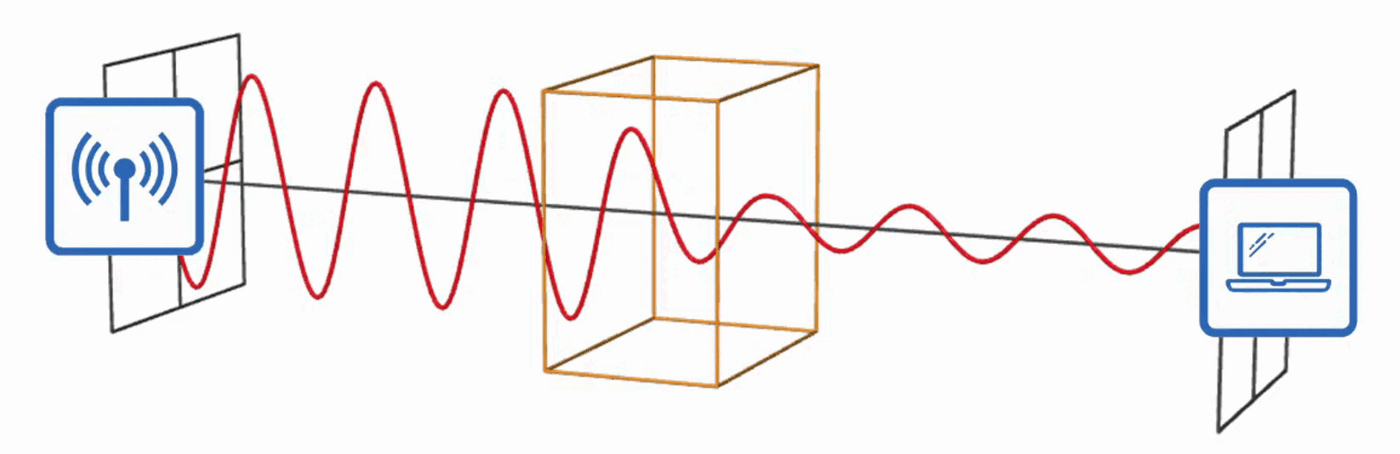
\includegraphics[keepaspectratio,alt={image}]{images/58-wireless-fundamentals/img-003.png}}
\end{figure}

\section{Signal Reflection}\label{signal-reflection}

\begin{itemize}
\tightlist
\item
  REFLECTION happens when a SIGNAL BOUNCES off a material (like metal)

  \begin{itemize}
  \tightlist
  \item
    This is why WI-FI reception is usually POOR in elevators. The SIGNAL
    bounces off the metal and very little penetrates into the elevator
  \end{itemize}
\end{itemize}

\begin{figure}
\centering
\pandocbounded{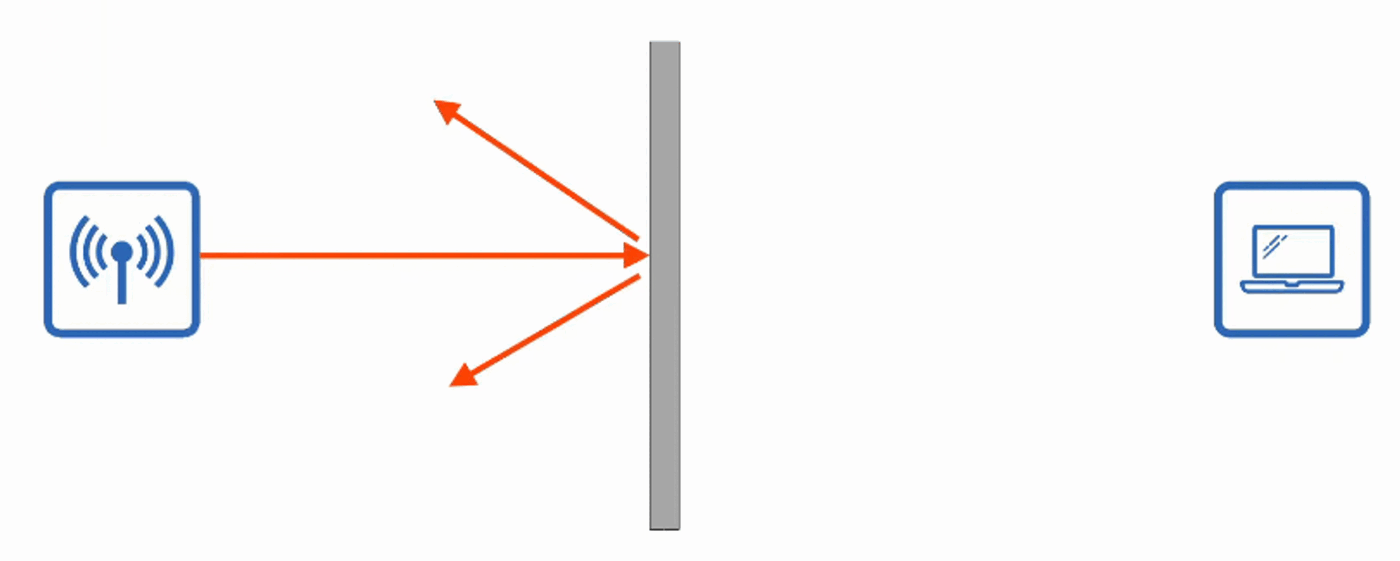
\includegraphics[keepaspectratio,alt={image}]{images/58-wireless-fundamentals/img-004.png}}
\end{figure}

\section{Signal Refraction}\label{signal-refraction}

\begin{itemize}
\tightlist
\item
  REFRACTION happens when a WAVE is BENT when entering a medium where
  the SIGNAL travels at a different speed

  \begin{itemize}
  \tightlist
  \item
    For example, glass and water can refract waves
  \end{itemize}
\end{itemize}

\begin{figure}
\centering
\pandocbounded{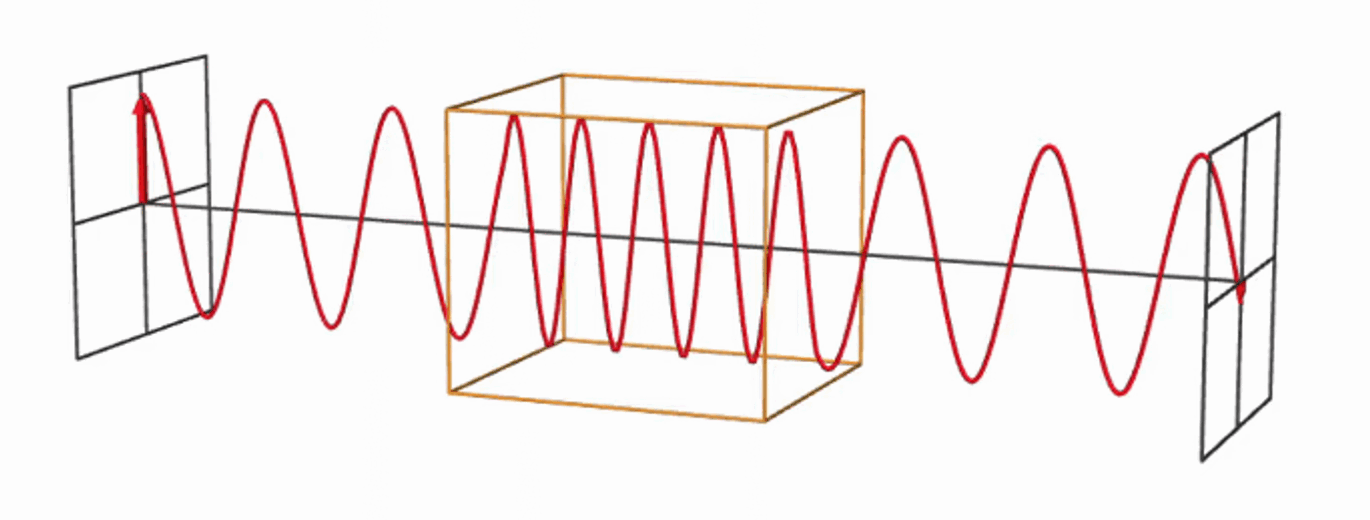
\includegraphics[keepaspectratio,alt={image}]{images/58-wireless-fundamentals/img-005.png}}
\end{figure}

\section{Signal Diffraction}\label{signal-diffraction}

\begin{itemize}
\tightlist
\item
  DIFFRACTION happens when a WAVE encounters an OBSTACLE and travels
  AROUND it

  \begin{itemize}
  \tightlist
  \item
    This can result in ``BLIND SPOTS'' behind the obstacle
  \end{itemize}
\end{itemize}

\begin{figure}
\centering
\pandocbounded{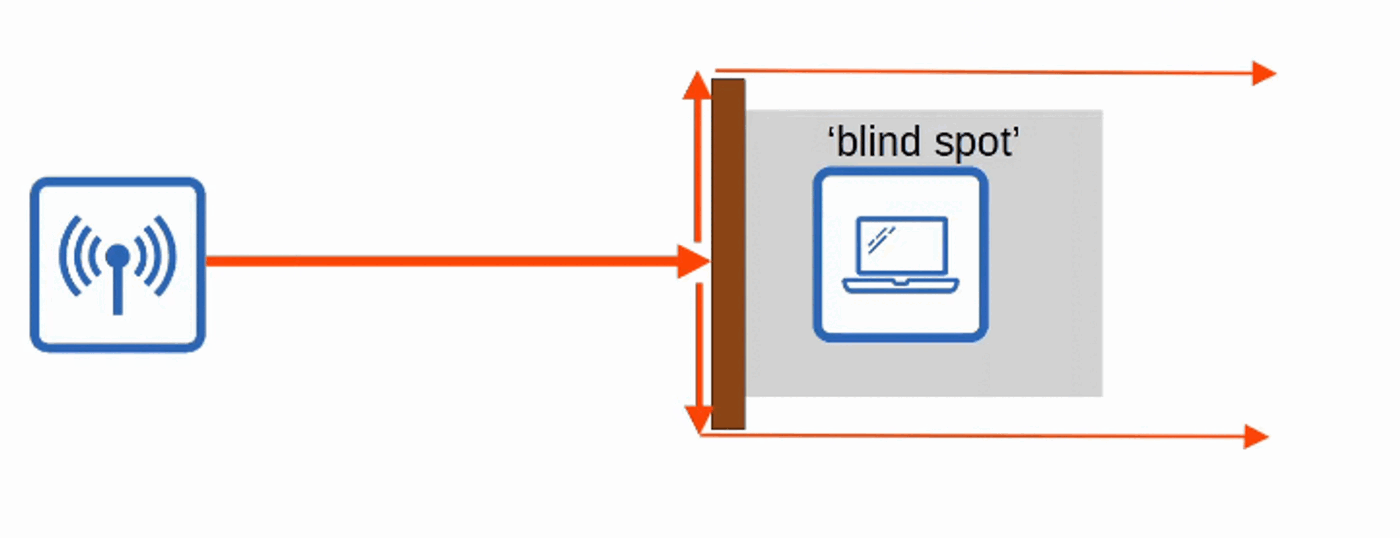
\includegraphics[keepaspectratio,alt={image}]{images/58-wireless-fundamentals/img-006.png}}
\end{figure}

\section{Signal Scattering}\label{signal-scattering}

\begin{itemize}
\tightlist
\item
  SCATTERING happens when a material causes a SIGNAL to SCATTER in all
  directions

  \begin{itemize}
  \tightlist
  \item
    Dust, smog, uneven surfaces, etc. can cause scattering
  \end{itemize}
\end{itemize}

\begin{figure}
\centering
\pandocbounded{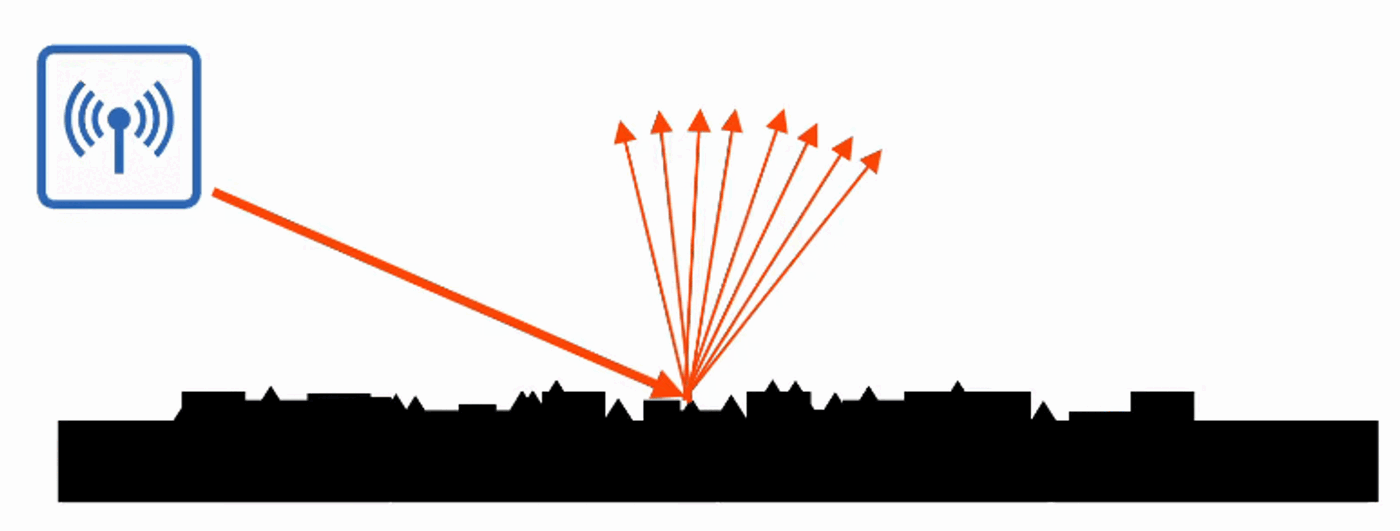
\includegraphics[keepaspectratio,alt={image}]{images/58-wireless-fundamentals/img-007.png}}
\end{figure}

\begin{enumerate}
\def\labelenumi{\arabic{enumi})}
\setcounter{enumi}{3}
\tightlist
\item
  Other DEVICES using the SAME CHANNELS can cause INTERFERENCE
\end{enumerate}

\begin{itemize}
\tightlist
\item
  For example, a WIRELESS LAN in your neighbor's house / apartment
\end{itemize}

\section{Radio Frequency (RF)}\label{radio-frequency-rf}

\begin{itemize}
\tightlist
\item
  To send WIRELESS SIGNALS, the SENDER applies an ALTERNATING CURRENT to
  an antenna

  \begin{itemize}
  \tightlist
  \item
    This creates ELECTROMAGNETIC WAVES which propagate out as WAVES
  \end{itemize}
\item
  ELECTROMAGENETIC WAVES can be measured in multiple ways - for example
  AMPLITUDE and FREQUENCY
\item
  AMPLITUDE is the MAXIMUM STRENGTH of the ELECTRIC and MAGNETIC FIELDS
\end{itemize}

\begin{figure}
\centering
\pandocbounded{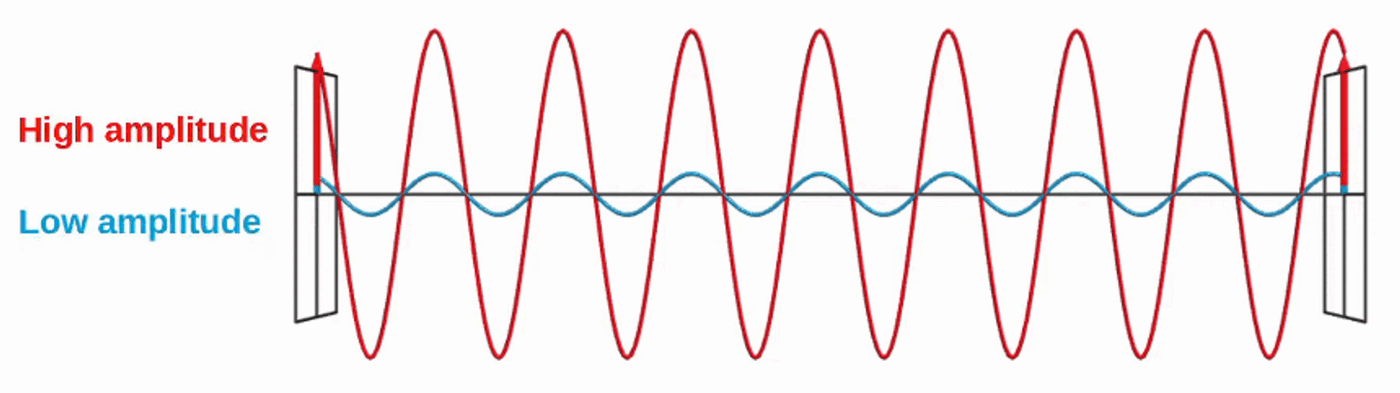
\includegraphics[keepaspectratio,alt={image}]{images/58-wireless-fundamentals/img-008.png}}
\end{figure}

\begin{itemize}
\tightlist
\item
  FREQUENCY measures the number of UP / DOWN CYCLES per a GIVEN UNIT of
  TIME
\item
  The most COMMON measurement of FREQUENCE is HERTZ

  \begin{itemize}
  \tightlist
  \item
    Hz (HERTZ) = cycles per second
  \item
    kHz (KILOHERZ) = 1,000 cycles per second
  \item
    MHz (MEGAHERZ) = 1,000,000 cycles per second
  \item
    GHz (GIGAHERTZ) = 1,000,000,000 cycles per second
  \item
    THz (TERAHERTZ) = 1,000,000,000,000 cycles per second
  \end{itemize}
\end{itemize}

4 CYCLES per 1 SECOND = 4 HERTZ

\begin{figure}
\centering
\pandocbounded{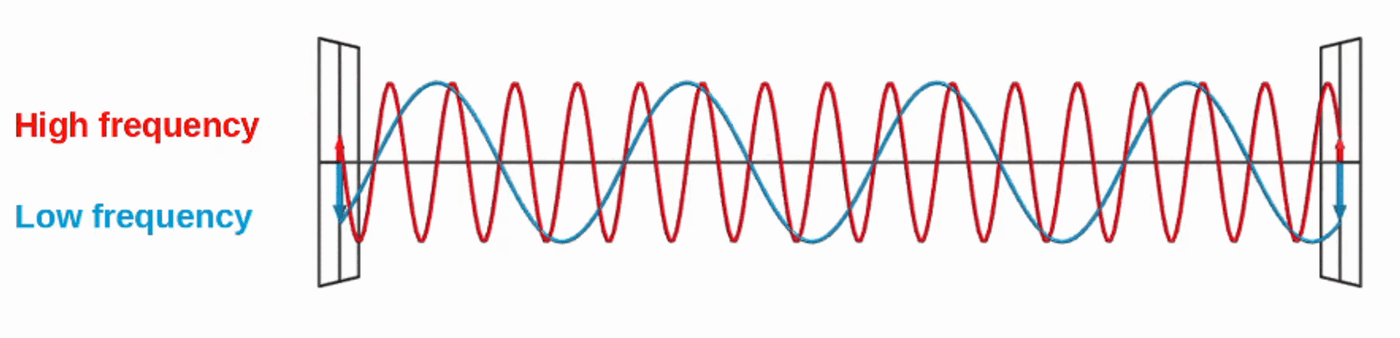
\includegraphics[keepaspectratio,alt={image}]{images/58-wireless-fundamentals/img-009.png}}
\end{figure}

\begin{figure}
\centering
\pandocbounded{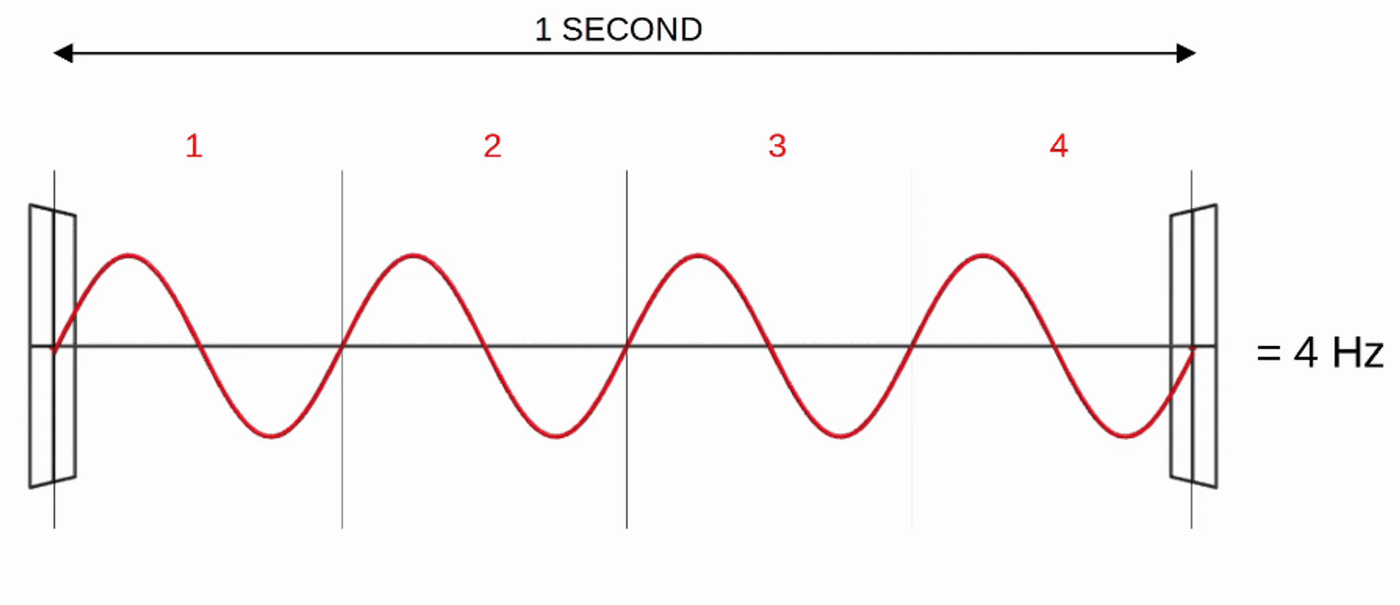
\includegraphics[keepaspectratio,alt={image}]{images/58-wireless-fundamentals/img-010.png}}
\end{figure}

\begin{itemize}
\tightlist
\item
  Another important term is PERIOD, the amount of TIME of ONE CYCLE

  \begin{itemize}
  \tightlist
  \item
    If the FREQUENCY is 4 Hz, the PERIOD is 0.25 SECONDS
  \end{itemize}
\end{itemize}

\begin{figure}
\centering
\pandocbounded{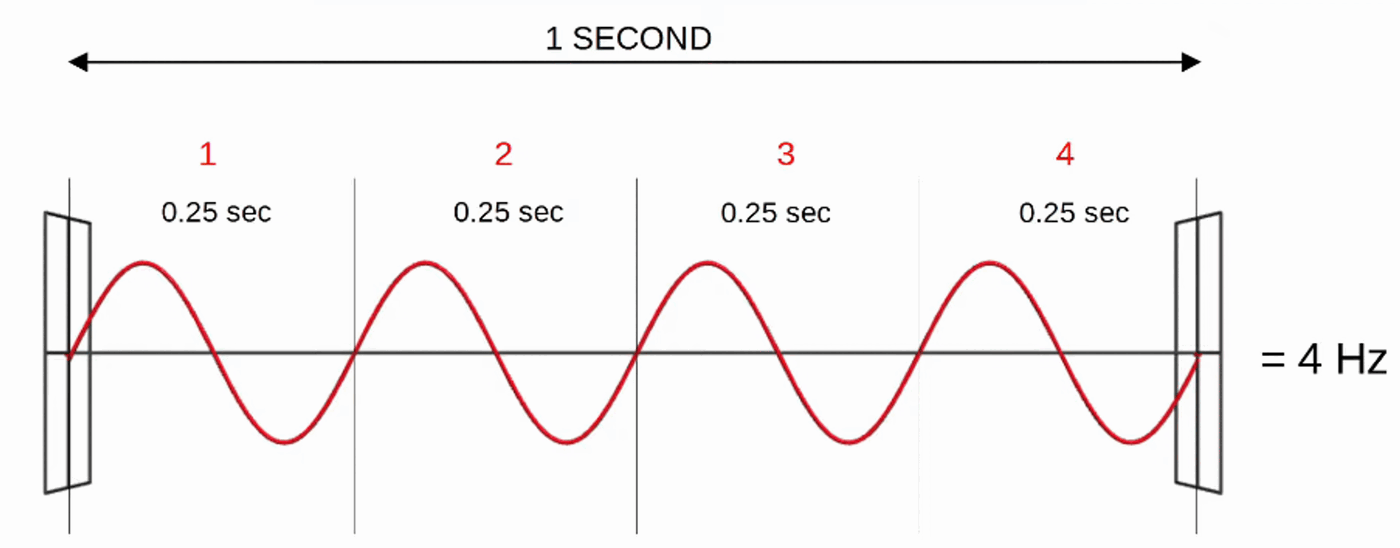
\includegraphics[keepaspectratio,alt={image}]{images/58-wireless-fundamentals/img-011.png}}
\end{figure}

\begin{itemize}
\tightlist
\item
  The VISIBLE FREQUENCY RANGE is \textasciitilde400 THz to 790 THz
\item
  The RADIO FREQUENCY RANGE is 30 Hz to 300 GHz and is used for many
  purposes.
\end{itemize}

\begin{figure}
\centering
\pandocbounded{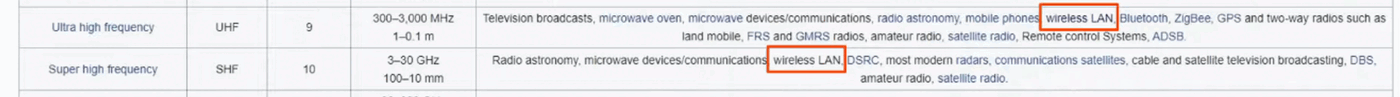
\includegraphics[keepaspectratio,alt={image}]{images/58-wireless-fundamentals/img-012.png}}
\end{figure}

\section{Radio Frequency Bands}\label{radio-frequency-bands}

\begin{itemize}
\tightlist
\item
  WI-FI uses TWO MAIN BANDS (FREQUENCY RANGES)
\item
  2.4 GHz band

  \begin{itemize}
  \tightlist
  \item
    Range is 2.400 - 2.4835 GHz
  \end{itemize}
\item
  5 GHz band

  \begin{itemize}
  \tightlist
  \item
    Range is 5.150 - 5.825 GHz
  \item
    Divided into FOUR SMALLER BANDS:

    \begin{itemize}
    \tightlist
    \item
      5.150 - 5.250 GHz
    \item
      5.250 - 5.350 GHz
    \item
      5.470 - 5.725 GHz
    \item
      5.725 - 5.825 GHz
    \end{itemize}
  \end{itemize}
\item
  The 2.4 GHz band typically provides FURTHER REACH in open space and
  BETTER PENETRATION of obstacles such as walls.

  \begin{itemize}
  \tightlist
  \item
    HOWEVER, more DEVICES tend to use the 2.4 GHz BAND so INTERFERENCE
    can be a BIGGER PROBLEM compared to 5GHz
  \end{itemize}
\end{itemize}

** WI-FI 6 (802.11ax) has EXPANDED the spectrum range to include a band
in the 6 GHz RANGE

\section{Channels}\label{channels}

\begin{itemize}
\tightlist
\item
  Each BAND is divided up into MULTIPLE ``CHANNELS''

  \begin{itemize}
  \tightlist
  \item
    DEVICES are configured to TRANSMIT and RECEIVE traffic on one (or
    more) of these CHANNELS
  \end{itemize}
\item
  The 2.4 GHz BAND is divided into several CHANNELS, each with a 22 MHz
  RANGE
\item
  In a SMALL WIRELESS LAN with only a single ACCESS POINT (AP), you can
  use ANY channel
\item
  However, in larger WLANs with multiple APs, it's important that
  adjacent APs don't use OVERLAPPING CHANNELS. This helps avoid
  INTERFERENCE
\item
  In the 2.4 GHz BAND, it is recommended to use CHANNELS 1, 6 and 11
\end{itemize}

\begin{figure}
\centering
\pandocbounded{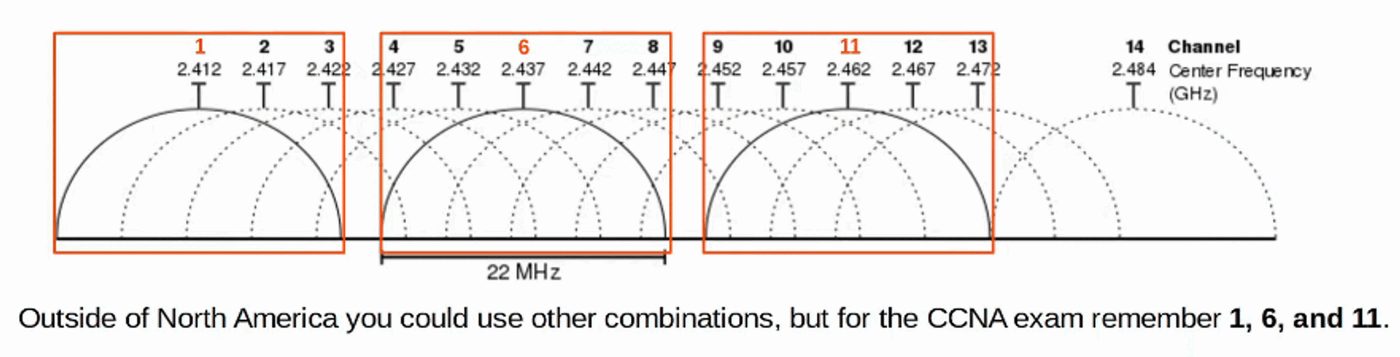
\includegraphics[keepaspectratio,alt={image}]{images/58-wireless-fundamentals/img-013.png}}
\end{figure}

\begin{itemize}
\item
  The 5 GHz BAND consists of NON-OVERLAPPING channels so it's much
  EASIER to avoid INTERFERENCE between adjacent APs
\item
  Using CHANNELS 1, 6, 11, you can place APs in a ``HONEYCOMB'' pattern
  to provide COMPLETE coverage of an area without INTERFERENCE between
  CHANNELS
\end{itemize}

\begin{figure}
\centering
\pandocbounded{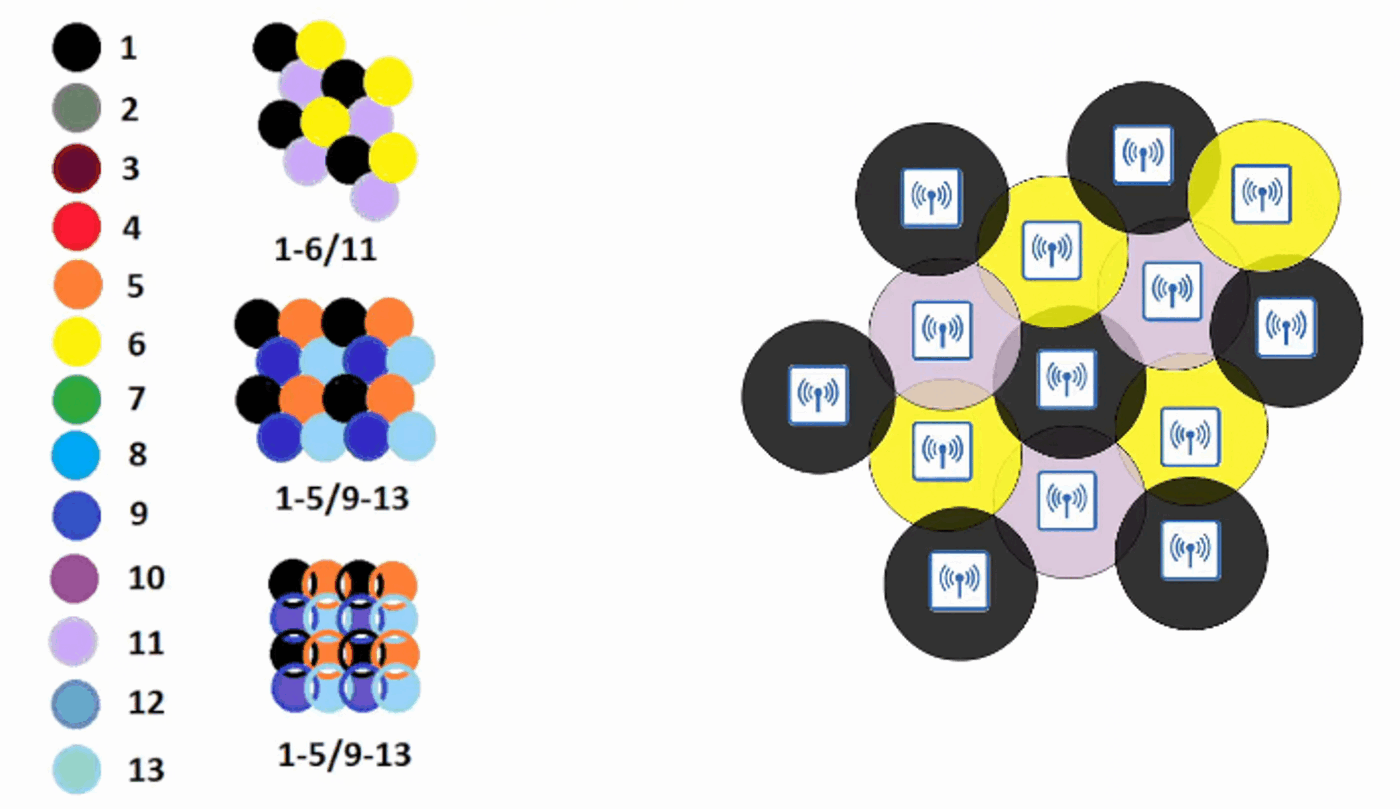
\includegraphics[keepaspectratio,alt={image}]{images/58-wireless-fundamentals/img-014.png}}
\end{figure}

\section{Wi-Fi Standards (802.11)}\label{wi-fi-standards-802.11}

\begin{figure}
\centering
\pandocbounded{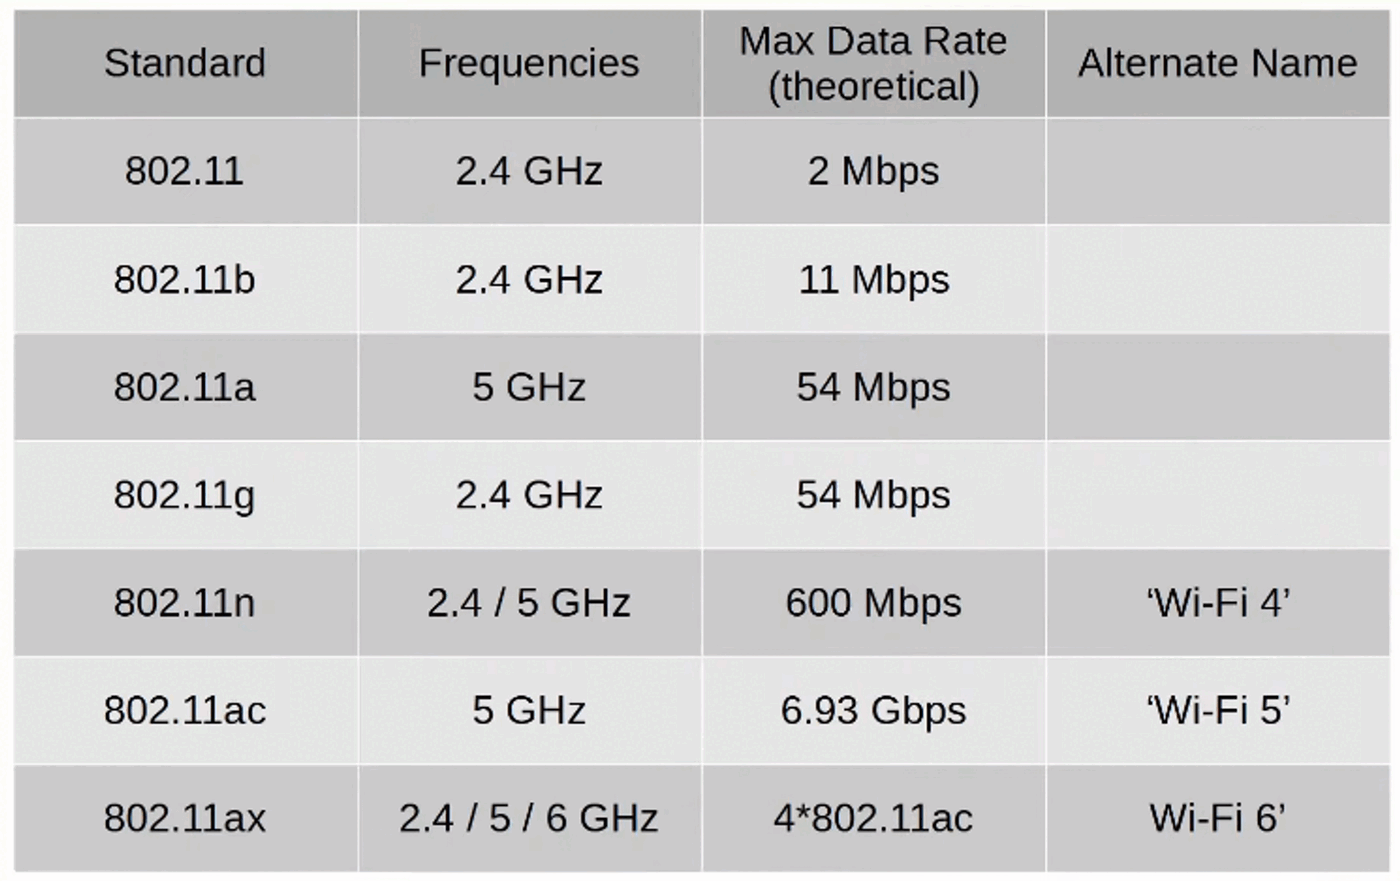
\includegraphics[keepaspectratio,alt={image}]{images/58-wireless-fundamentals/img-015.png}}
\end{figure}

\section{Service Sets}\label{service-sets}

\begin{itemize}
\tightlist
\item
  802.11 defines different kinds of SERVICE SETS which are groups of
  WIRELESS NETWORK DEVICES
\item
  There are THREE MAIN TYPES:

  \begin{itemize}
  \tightlist
  \item
    INDEPENDENT
  \item
    INFRASTRUCTURE
  \item
    MESH
  \end{itemize}
\item
  ALL DEVICES in a SERVICE SET share the same SSID (Service Set
  Identifier)
\item
  The SSID is a HUMAN-READABLE NAME which identifies the SERVICE SET
\item
  The SSID does NOT have to be UNQUE
\end{itemize}

\section{Service Sets : IBSS}\label{service-sets-ibss}

\begin{itemize}
\tightlist
\item
  An IBSS (INDEPENDENT BASIC SERVICE SET) is a WIRELESS NETWORK in which
  TWO or MORE WIRELESS DEVICES connect directly without using an AP
  (ACCESS POINT)
\item
  Also called an AD HOC NETWORK
\item
  Can be used for FILE TRANSFER (ie: AirDrop)
\item
  Not scalable beyond a few DEVICES
\end{itemize}

\begin{figure}
\centering
\pandocbounded{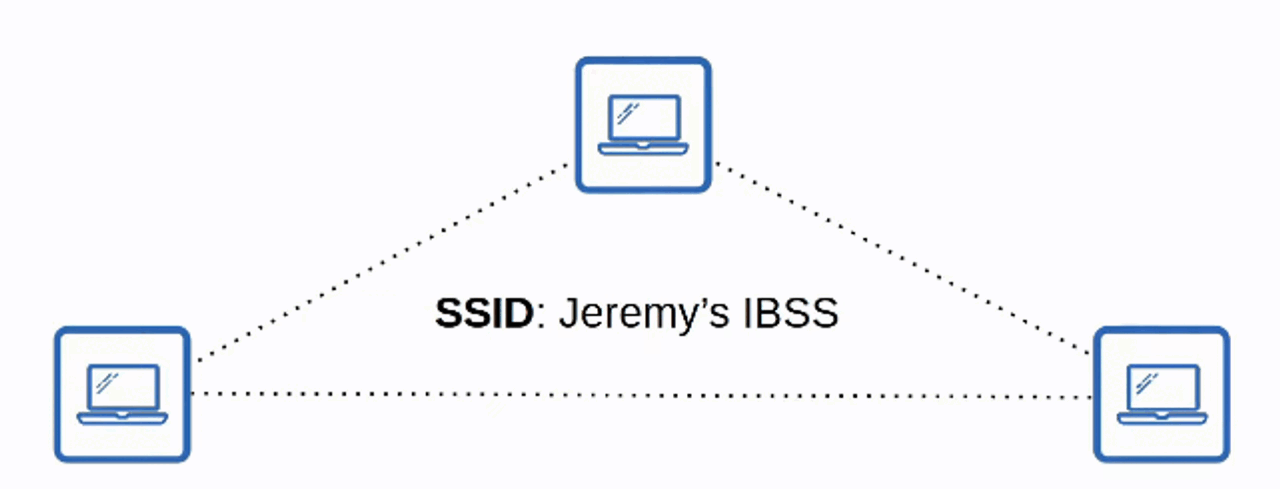
\includegraphics[keepaspectratio,alt={image}]{images/58-wireless-fundamentals/img-016.png}}
\end{figure}

\section{Service Sets : BSS}\label{service-sets-bss}

\begin{itemize}
\tightlist
\item
  A BSS (BASIC SERVICE SET) is a kind of infrastructure SERVICE SET in
  which CLIENTS connect to each other via an AP (ACCESS POINT) but not
  DIRECTLY to each other
\item
  A BSSID (BASIC SERVICE SET ID) is used to uniquely identify the AP

  \begin{itemize}
  \tightlist
  \item
    Other APs can use the SAME SSID but NOT THE SAME BSSID
  \item
    The BSSID is the MAC ADDRESS of the APs RADIO
  \end{itemize}
\item
  WIRELESS DEVICES request to \emph{associate} with the BSS
\item
  WIRELESS DEVICES that have associated with the BSS are called
  ``CLIENTS'' or ``STATIONS''
\item
  The AREA around an AP where its SIGNAL is usable is called a BSA
  (BASIC SERVICE AREA)
\end{itemize}

\begin{figure}
\centering
\pandocbounded{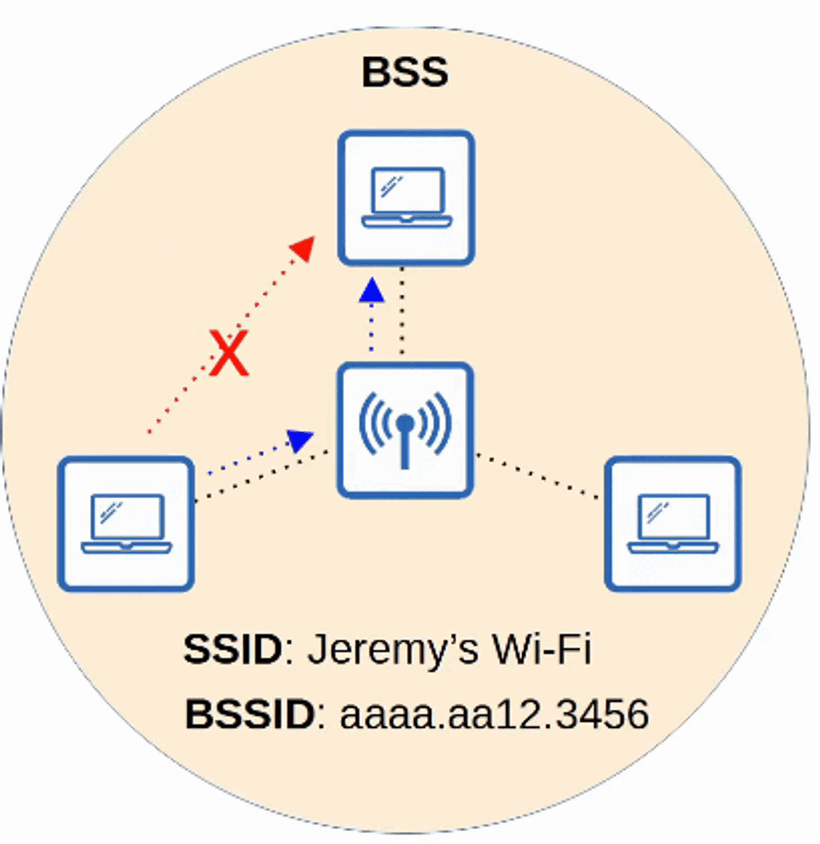
\includegraphics[keepaspectratio,alt={image}]{images/58-wireless-fundamentals/img-017.png}}
\end{figure}

\section{Service Sets: ESS}\label{service-sets-ess}

\begin{itemize}
\tightlist
\item
  To create LARGER WIRELESS LANS beyond the range of a SINGLE AP, we use
  an ESS (EXTENDED SERVICE SET)
\item
  APs with their own BSSs are connected by a WIRED NETWORK

  \begin{itemize}
  \tightlist
  \item
    Each BSS uses the SAME SSID
  \item
    Each BSS has a UNIQUE BSSID
  \item
    Each BSS uses a DIFFERENT channel to avoid INTERFERENCE
  \end{itemize}
\item
  CLIENTS can pass between APs without having to RECONNECT, providing a
  SEAMLESS WI-FI experience when moving between APs

  \begin{itemize}
  \tightlist
  \item
    This is called ROAMING
  \end{itemize}
\item
  The BSAs should overlap about 10-15\%
\end{itemize}

\begin{figure}
\centering
\pandocbounded{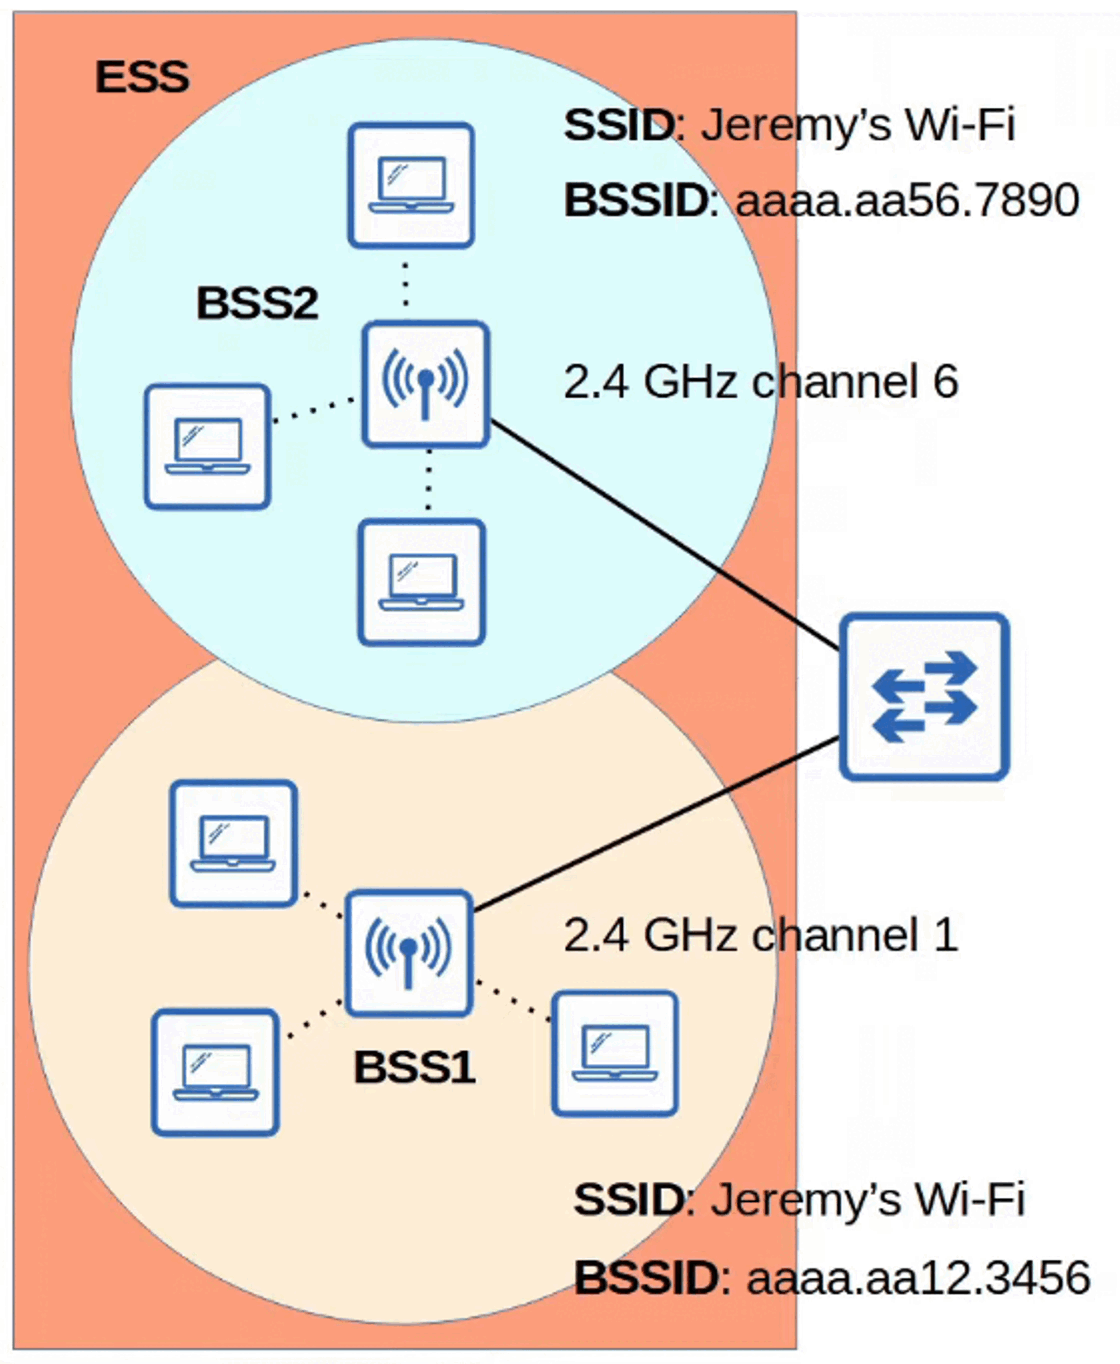
\includegraphics[keepaspectratio,alt={image}]{images/58-wireless-fundamentals/img-018.png}}
\end{figure}

\section{Service Sets: MBSS}\label{service-sets-mbss}

\begin{itemize}
\tightlist
\item
  An MBSS (MESH BASIC SERVICE SET) can be used in situations where it's
  difficult to run an ETHERNET connection to every AP
\item
  MESH APs use TWO RADIOS:

  \begin{itemize}
  \tightlist
  \item
    ONE provides BSS to WIRELESS CLIENTS
  \item
    ONE forms a ``BACKHAUL NETWORK'' which is used to BRIDGE traffic
    from AP to AP
  \end{itemize}
\item
  At least ONE AP is connected to the WIRED NETWORK and it is called the
  RAP (ROOT ACCESS POINT)
\item
  The OTHER APs are called MAPs (MESH ACCESS POINTS)
\item
  A PROTOCOL is used to determine the BEST PATH through the MESH
  (similar to how DYNAMIC ROUTING PROTOCOLS are used to determine the
  BEST PATH to a DESTINATION)
\end{itemize}

\begin{figure}
\centering
\pandocbounded{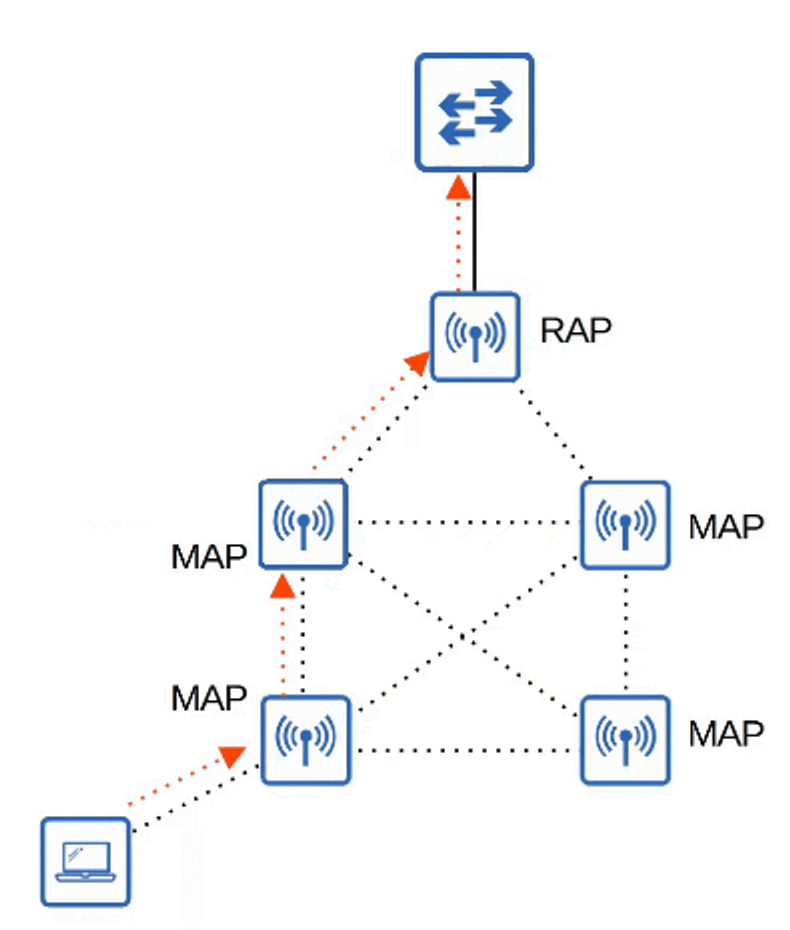
\includegraphics[keepaspectratio,alt={image}]{images/58-wireless-fundamentals/img-019.png}}
\end{figure}

\section{Distribution System}\label{distribution-system}

\begin{itemize}
\tightlist
\item
  Most WIRELESS NETWORKS are not STANDALONE NETWORKS

  \begin{itemize}
  \tightlist
  \item
    Rather, they are a way for WIRELESS CLIENTS to connect to the WIRED
    NETWORK INFRASTRUCTURE
  \end{itemize}
\item
  In 802.11, the UPSTREAM WIRED NETWORK is called the DS (DISTRIBUTION
  SYSTEM)
\item
  Each WIRELESS BSS or ESS is mapped to a VLAN in the WIRED NETWORK
\end{itemize}

\begin{figure}
\centering
\pandocbounded{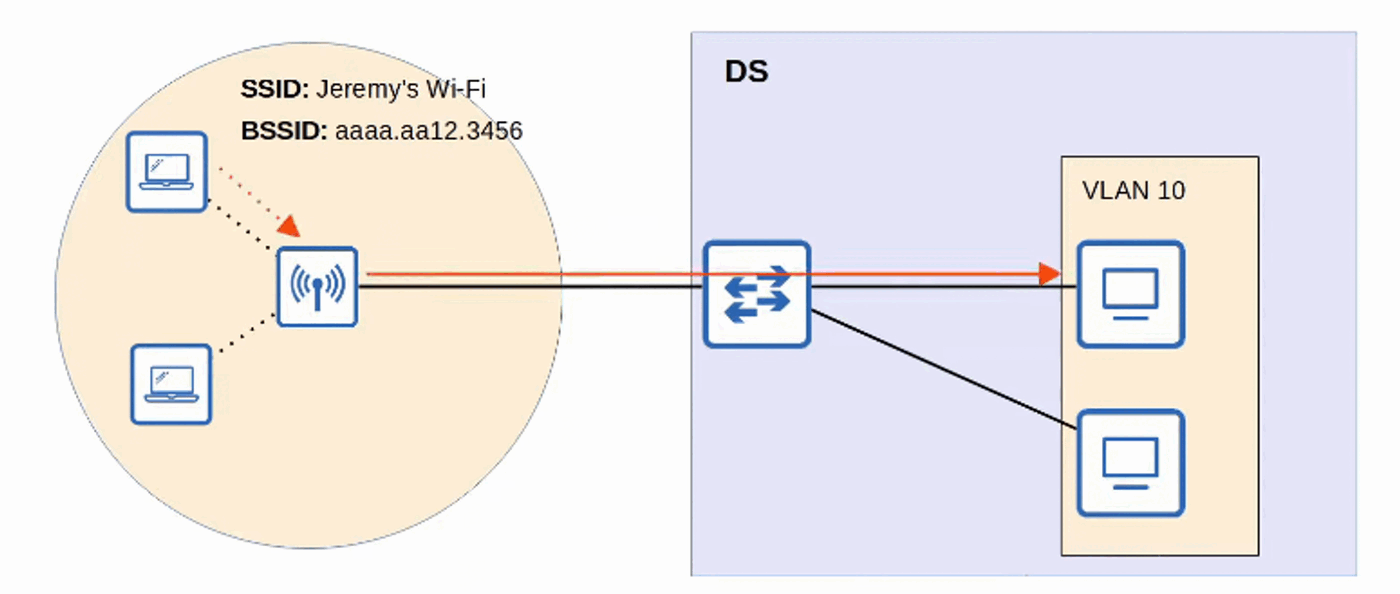
\includegraphics[keepaspectratio,alt={image}]{images/58-wireless-fundamentals/img-020.png}}
\end{figure}

\begin{itemize}
\tightlist
\item
  It is possible for an AP to provide MULTIPLE WIRELESS LANs, each with
  a unique SSID
\item
  Each WLAN is mapped to a separate VLAN and connected to the WIRED
  NETWORK via a TRUNK
\item
  Each WLAN uses a UNIQUE BSSID, usually by INCREMENTING the LAST digit
  of the BBSID by one
\end{itemize}

\begin{figure}
\centering
\pandocbounded{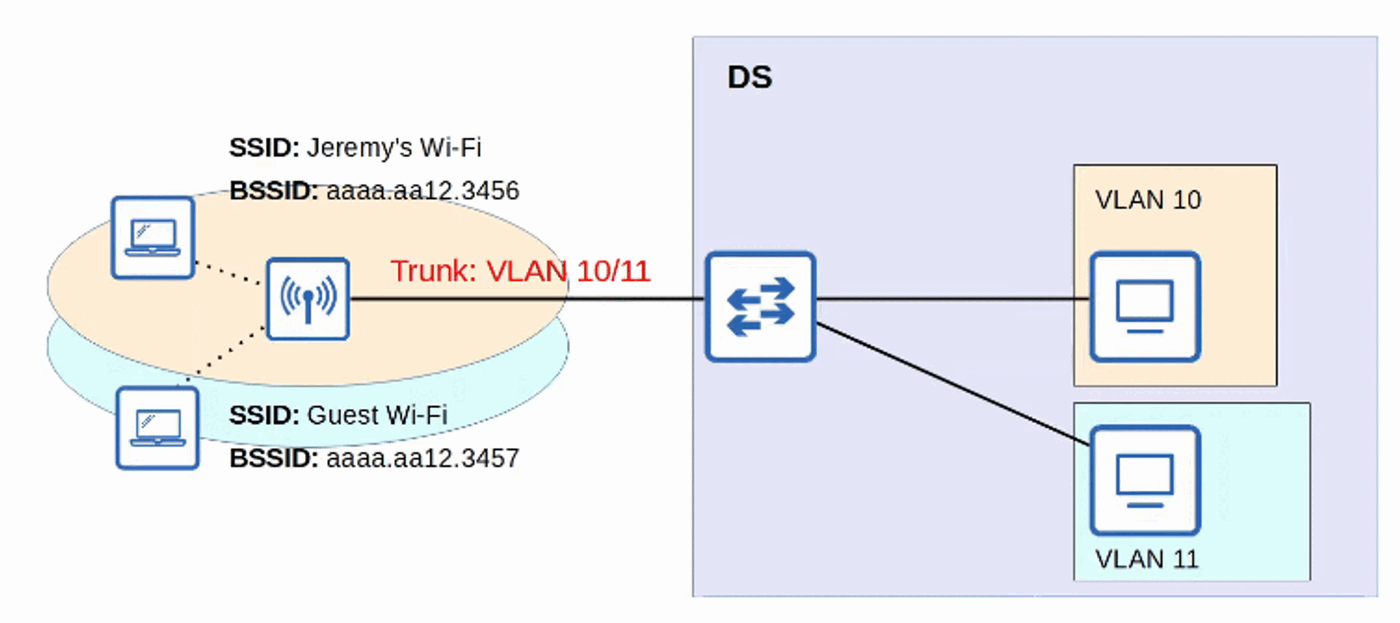
\includegraphics[keepaspectratio,alt={image}]{images/58-wireless-fundamentals/img-021.png}}
\end{figure}

\section{Additional AP Operational
Modes}\label{additional-ap-operational-modes}

\begin{itemize}
\item
  APs can operate in ADDITIONAL MODES beyond the ones we've introduced
  so far
\item
  An AP in REPEATER MODE can be used to EXTEND the RANGE of a BSS
\item
  The REPEATER will re-transmit ANY SIGNAL it receives from the AP

  \begin{itemize}
  \tightlist
  \item
    A REPEATER with a SINGLE RADIO must operate on the SAME CHANNEL as
    the AP, but this can drastically reduce the overall THROUGHPUT on
    the CHANNEL
  \item
    A REPEATER with TWO RADIOS can receive on ONE CHANNEL and then
    retransmit on ANOTHER CHANNEL
  \end{itemize}
\end{itemize}

\begin{figure}
\centering
\pandocbounded{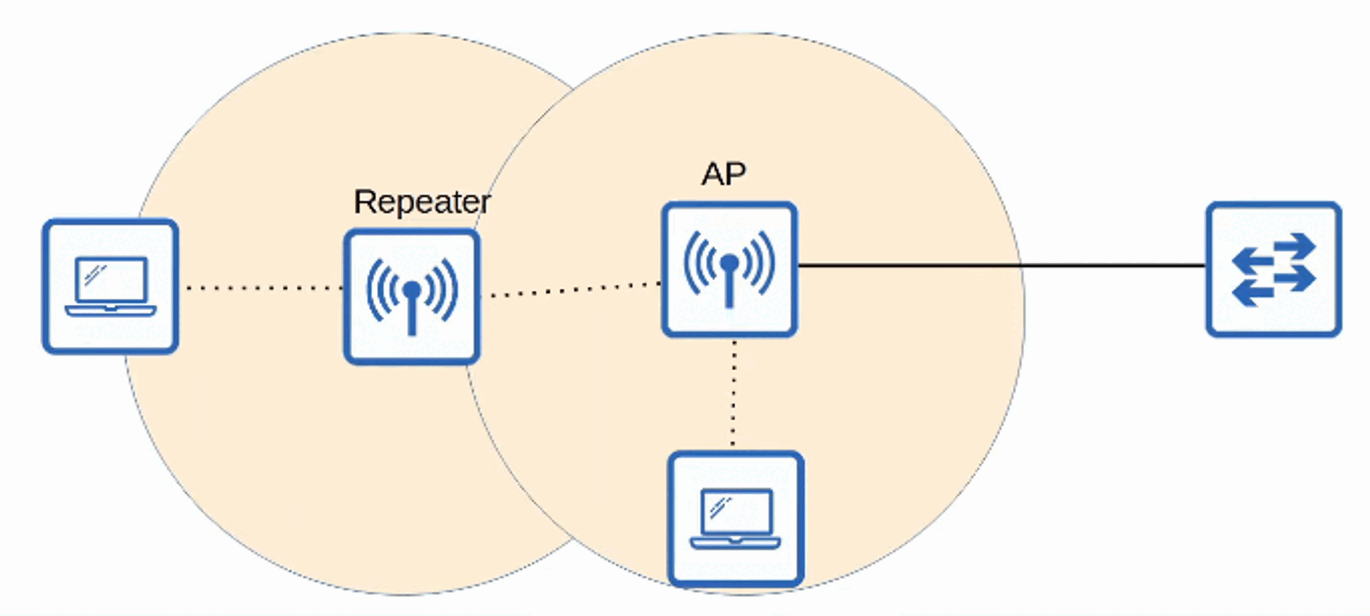
\includegraphics[keepaspectratio,alt={image}]{images/58-wireless-fundamentals/img-022.png}}
\end{figure}

\begin{itemize}
\tightlist
\item
  A WORKGROUP BRIDGE (WGB) operates as a WIRELESS CLIENT of another AP
  and can be used to CONNECT WIRED DEVICES to the WIRELESS NETWORK
\item
  In the example below, PC1 does NOT have WIRELESS CAPABILITIES, and
  also DOES NOT have ACCESS to WIRED CONNECTIONS to SW1
\item
  PC1 has a WIRED CONNECTION to the WGB, which has a WIRELESS CONNECTION
  to the AP
\end{itemize}

\begin{figure}
\centering
\pandocbounded{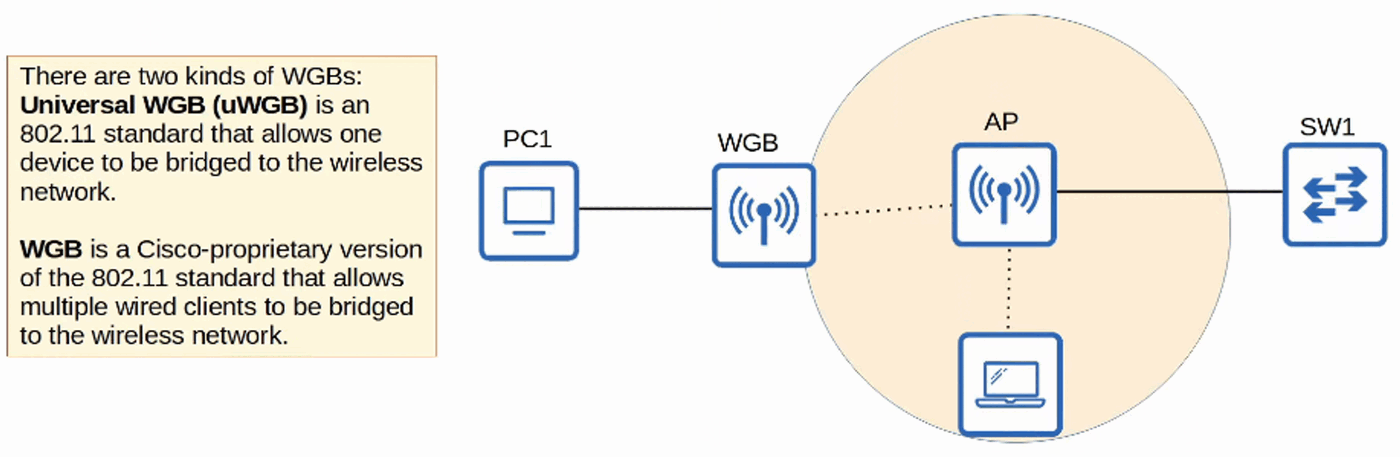
\includegraphics[keepaspectratio,alt={image}]{images/58-wireless-fundamentals/img-023.png}}
\end{figure}

\begin{itemize}
\tightlist
\item
  AN OUTDOOR BRIDGE can be used to connect NETWORKS over LONG DISTANCES
  without a PHYSICAL CABLE connecting them
\item
  The APs will use SPECIALIZED ANTENNAS that focus most of the SIGNAL
  POWER in one direction, which allows the WIRELESS CONNECTION to be
  made over LONGER DISTANCES than normally possible
\item
  The CONNECTION can be POINT-TO-POINT as in the diagram below, or
  POINT-TO-MULTIPOINT in which MULTIPLE SITES connect to on CENTRAL SITE
\end{itemize}

\begin{figure}
\centering
\pandocbounded{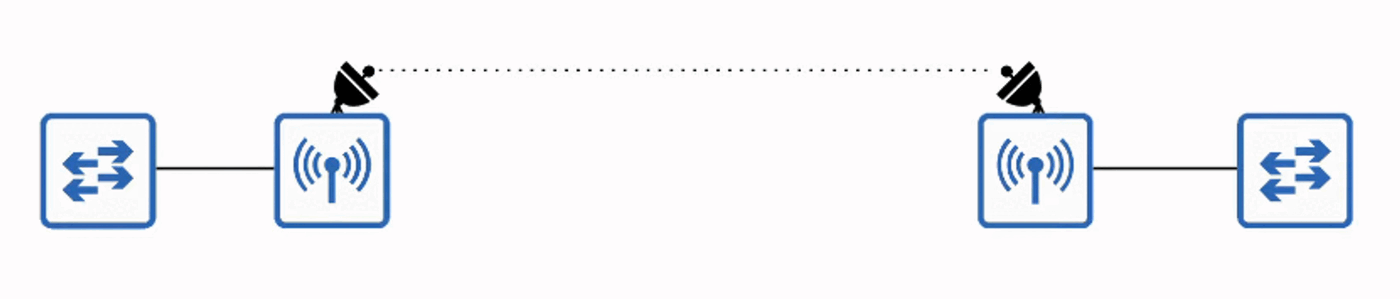
\includegraphics[keepaspectratio,alt={image}]{images/58-wireless-fundamentals/img-024.png}}
\end{figure}

REVIEW
\pandocbounded{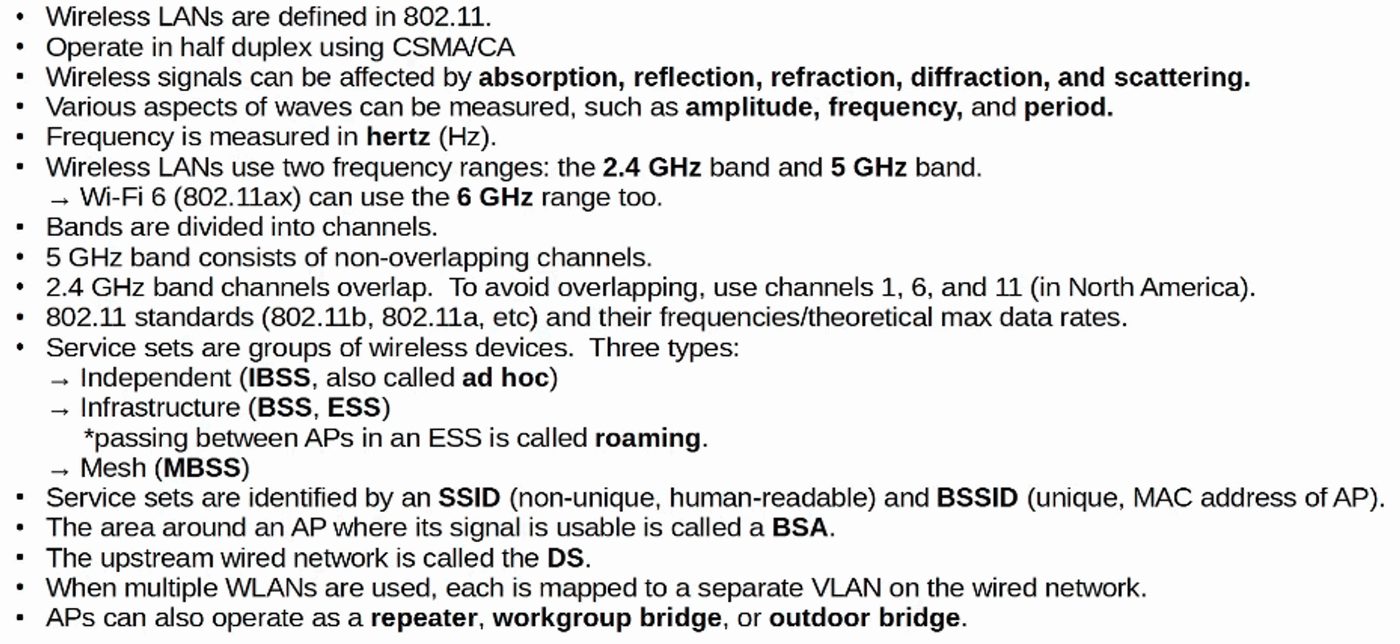
\includegraphics[keepaspectratio,alt={image}]{images/58-wireless-fundamentals/img-025.png}}
